
\documentclass[11pt, a4paper]{book}
% Ressources à installer : texlive-science et texlive-lang-french ou texlive-lang-european
%à compiler avec XeLaTeX à cause des image pstricks

\usepackage[utf8]{inputenc}
\usepackage[T1]{fontenc}

\usepackage[french]{babel}
\usepackage{listingsutf8}
\usepackage{pdfpages}
\usepackage{tikz,pgf}
\usepackage{amsthm,titlesec}
\usepackage{mdframed} % pour le format des définition, théorèmes...
\usepackage{xcolor,rotating,systeme}
\usepackage[Glenn]{fncychap} %pour le format des chapitres
\usepackage[top=3cm,bottom=3cm,left=3cm,right=2cm,headsep=10pt,a4paper]{geometry} % Page margins
\usepackage{multicol}
\usepackage{comment}
\usepackage{enumerate,cancel}
\usepackage{lipsum,minitoc}
%\usepackage{chngcntr}
\usepackage{amsmath,amsfonts,minitoc,amsthm,pgfplots}
\usepackage{mathrsfs}
\usetikzlibrary{arrows, intersections}
\usepackage{mathrsfs}
\usepackage{array,yhmath}
\usepackage{hyperref}
\usepackage{caption}
\usepackage{float}
\usepackage{wrapfig}
\restylefloat{figure}
%\usepackage{subfig}

\usepackage{subcaption}

\usepackage{listings}
\usepackage{color}
\lstset{ % General setup for the package
    language=Python,
    basicstyle=\footnotesize,
    basewidth=0.7em,
    numbers=left,
     numberstyle=\tiny,
    frame=lines,
    tabsize=4,
    columns=fixed,
    showstringspaces=false,
    showtabs=false,
    keepspaces,
    commentstyle=\color{gray},
    keywordstyle=\color{blue},
    stringstyle=\color{magenta},
    inputencoding=utf8/latin1,
            extendedchars=true,
            literate=%
            {é}{{\'{e}}}1
            {è}{{\`{e}}}1
            {ê}{{\^{e}}}1
            {ë}{{\¨{e}}}1
            {û}{{\^{u}}}1
            {ù}{{\`{u}}}1
            {â}{{\^{a}}}1
            {à}{{\`{a}}}1
            {î}{{\^{i}}}1
            {ô}{{\^{o}}}1
            {ç}{{\c{c}}}1
            {Ç}{{\c{C}}}1
            {É}{{\'{E}}}1
            {Ê}{{\^{E}}}1
            {À}{{\`{A}}}1
            {Â}{{\^{A}}}1
            {Î}{{\^{I}}}1
    }



\usepackage{lipsum}
\newtheorem{example}{Exemple}

\usepackage{pstricks,pst-plot,pstricks-add}
\usepackage{pst-func,tkz-tab,tkz-euclide}
\usepackage{graphicx}
%macro exo
\newcounter{mtex}[chapter]
\newcommand{\mtexlabel}{\cadrexo{\themtex}}
\newcommand{\cadrexo}[1]{%
\tikz\node[rectangle,minimum size=6mm,rounded corners=2mm,fill=ocre,inner sep=0pt,text width=0.8cm,align=center]{\large\bfseries\textcolor{white}{#1}};}
\definecolor{ocre}{RGB}{196,106,106}
\definecolor{vert}{RGB}{55,120,0}
\newcommand{\mtexlabelpos}[1]{%
\makebox[0pt][r]{\raisebox{#1\baselineskip}[0pt][0pt]{\mtexlabel\quad}}}
\newenvironment{exercice}[1][\empty]{%
\refstepcounter{mtex}%
\trivlist\item\relax%  
\ifx#1\empty\mtexlabelpos{-.7}\else\mtexlabelpos{-.5}%
\hfill\textbf{#1}\hfill\mbox{}\par\fi%
}{\endtrivlist}

\newcommand{\N}{\mathbb{N}}
\newcommand{\Z}{\mathbb Z}
\newcommand{\Q}{\mathbb Q}
\newcommand{\R}{\mathbb R}
\newcommand{\C}{\mathbb C}

\newcommand{\ssi}{\;\;\Leftrightarrow\;\;}

\newcommand{\point}[1]{-- +(#1,#1) -- +(-#1,-#1) -- +(0,0) -- +(-#1,#1) -- +(#1,-#1)} 


\newcommand{\parallele}{\mathbin{\!/\mkern-5mu/\!}} %signe parallèle

\titleformat{\chapter}[frame]
{\setlength\fboxrule{2.25pt}\color{black}}%
{\filleft\scshape\LARGE%
\enspace  Chapitre \thechapter\enspace}%
{20pt}
{\rule{0pt}{30pt}\Huge\scshape\filleft}

\newcommand\fonction[5]{
$\begin{array}{rrll}
#1: & #2 & \rightarrow & #3 \\
  & #4 & \mapsto & #5
\end{array}$
}

%\titleformat
%{\section} % command
%[hang] % shape
%{\bfseries\Large} % format
%{ \thesection\quad} % label
%{0em} % sep
%{
%} % before-code
%[
%\vspace{-1ex}%
%\textcolor{blue!60}{\rule{10cm}{3pt}}
%] % after-code


%\theoremstyle{break}
\newtheoremstyle{definition-style}  %style des theoreme
{}               
{}               
{}                   
{}                   
{\bf\sffamily} 
{~:\\[0.3cm]}                 
{.5em}               
{\thmname{#1}\thmnumber{ #2}\thmnote{ (#3)}}

\mdfdefinestyle{defi-frame}{
linewidth=10pt, %
linecolor= blue!50, % 
backgroundcolor= blue!20,
topline=false, %
bottomline=false, %
rightline=false,%
leftmargin=0pt, %
innerleftmargin=15pt, %
innerrightmargin=1em, 
rightmargin=0pt, % 
innertopmargin=-2pt,%
innerbottommargin=6pt, % 
splittopskip=\topskip, %
%splitbottomskip=\topskip, %
}% 

\mdfdefinestyle{methode-frame}{
	linewidth=10pt, %
linecolor= gray!70, % 
backgroundcolor= white,
topline=false, %
bottomline=false,%
rightline=false,%
leftmargin=0pt, %
innerleftmargin=15pt, %
innerrightmargin=1em, 
rightmargin=0pt, % 
innertopmargin=-2pt,%
innerbottommargin=6pt, % 
splittopskip=\topskip, %
%splitbottomskip=\topskip, %
}% 


\mdfdefinestyle{thm-frame}{
linewidth=10pt, %
linecolor= red!50, % 
backgroundcolor= orange!30,
topline=false, %
bottomline=false, %
rightline=false,%
leftmargin=0pt, %
innerleftmargin=15pt, %
innerrightmargin=1em, 
rightmargin=0pt, % 
innertopmargin=-2pt,%
innerbottommargin=6pt, % 
splittopskip=\topskip, %
%splitbottomskip=\topskip, %
}% 

\mdfdefinestyle{lem-frame}{
linewidth=10pt, %
linecolor= yellow!50, % 
backgroundcolor= yellow!10,
topline=false, %
bottomline=false, %
rightline=false,%
leftmargin=0pt, %
innerleftmargin=15pt, %
innerrightmargin=1em, 
rightmargin=0pt, % 
innertopmargin=-2pt,%
innerbottommargin=6pt, % 
splittopskip=\topskip, %
%splitbottomskip=\topskip, %
}% 

\mdfdefinestyle{notation-frame}{
linewidth=10pt, %
linecolor= blue!30, % 
backgroundcolor= blue!10,
topline=false, %
bottomline=false, %
rightline=false,%
leftmargin=0pt, %
innerleftmargin=15pt, %
innerrightmargin=1em, 
rightmargin=0pt, % 
innertopmargin=-2pt,%
innerbottommargin=6pt, % 
splittopskip=\topskip, %
%splitbottomskip=\topskip, %
}% 

\mdfdefinestyle{remarque-frame}{
linewidth=0pt, %
linecolor= black!0, % 
backgroundcolor= blue!0,
topline=false, %
bottomline=false, %
rightline=false,%
leftmargin=0pt, %
innerleftmargin=25pt, %
innerrightmargin=25pt, 
rightmargin=0pt, % 
innertopmargin=-2pt,%
innerbottommargin=6pt, % 
splittopskip=\topskip, %
%splitbottomskip=\topskip, %
}% 
\surroundwithmdframed[style=defi-frame]{defi}

\surroundwithmdframed[style=thm-frame]{thm}

\surroundwithmdframed[style=lem-frame]{lem}

\surroundwithmdframed[style=notation-frame]{notation}

\surroundwithmdframed[style=remarque-frame]{remarque}

\surroundwithmdframed[style=remarque-frame]{remarques}

\surroundwithmdframed[style=methode-frame]{methode}

\theoremstyle{definition-style}

%pour avoir un compteur commun a remarque et remarques
\newcounter{compteurremarque}[chapter]
\renewcommand{\thecompteurremarque}{\arabic{compteurremarque}} %définition de l'affichage du compteur

\newtheorem{defi}{Définition}[chapter]
\renewcommand{\thedefi}{\arabic{defi}} %pour ne pas avoir le numéro du chapitre dans la numération de la def
\newtheorem{thm}{Théorème}[chapter]
\renewcommand{\thethm}{\arabic{thm}}
\newtheorem{lem}{Lemme}[chapter]
\renewcommand{\thelem}{\arabic{lem}}
\newtheorem{notation}{Notation}[chapter]
\renewcommand{\thenotation}{\arabic{notation}}
%\newtheorem{remarque}{Remarque}[chapter]
%\renewcommand{\theremarque}{\arabic{remarque}}
%\newtheorem{remarques}{Remarques}[chapter]
%\renewcommand{\theremarques}{\arabic{remarques}}
\newtheorem{methode}{Méthode}[chapter]
\renewcommand{\themethode}{\arabic{methode}}


\newtheorem{remarque}[compteurremarque]{Remarque}
\newtheorem{remarques}[compteurremarque]{Remarques} %remarque et remarques prennent compteurremarque comme compteur commun

\lstMakeShortInline[columns=fixed]|

%%%%%%%% Commandes de Matthieu

%-------------------------------------------------------------------------------
%---- Eclairage : en encadré sur fond jaune avec symbôle "ampoule" à gauche ----
%-------------------------------------------------------------------------------
\definecolor{coleclairage}{RGB}{255 , 221 , 156}
\definecolor{contoureclairage}{RGB}{255 , 192 , 0}
\newenvironment{eclairage}
{
	\begin{center}%
		\begin{tikzpicture}%
			\node[rectangle, draw=contoureclairage, top color=coleclairage!50, bottom color=coleclairage!140, rounded corners=5pt, inner xsep=5pt, inner ysep=6pt, outer ysep=10pt]\bgroup                     
			\begin{minipage}{0.98\linewidth}
				\begin{minipage}{0.08\linewidth}\centerline{
\includegraphics[scale=1]{images/Symbole_eclairage.png}}\end{minipage}
				\begin{minipage}{0.89\linewidth}\itshape\footnotesize
				}
				{                		
				\end{minipage}
			\end{minipage}\egroup;%
		\end{tikzpicture}%
	\end{center}%
}



\newcommand{\putfigure}[6]{
    \begin{minipage}{#1\textwidth}
    \centering
        \includegraphics[width=#2\textwidth,height=#3\textheight]{#4}
        \captionof{figure}{#5}
        \label{#6}
    \end{minipage}
}


\newcommand{\itemb}[1]{\item \textbf{#1}}



%-------------------------------------------------------------------------------
%---- apprendre : en encadré sur fond jaune avec symbole "ampoule" à gauche ----
%-------------------------------------------------------------------------------
\definecolor{colapprendre}{RGB}{50,205,50}
\definecolor{contourapprendre}{RGB}{34,139,34}
\newenvironment{apprendre}
{
	\begin{center}%
		\begin{tikzpicture}%
			\node[rectangle, draw=contourapprendre, top color=colapprendre!10, bottom color=colapprendre!50, rounded corners=5pt, inner xsep=5pt, inner ysep=6pt, outer ysep=10pt]\bgroup                     
			\begin{minipage}{0.98\linewidth}
				\begin{minipage}{0.08\linewidth}\centerline{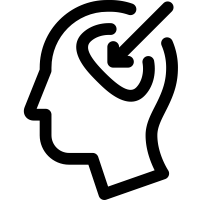
\includegraphics[width=30px]{images/Symbole_learn.png}}\end{minipage}
				\begin{minipage}{0.89\linewidth}\itshape\footnotesize
				}
				{                		
				\end{minipage}
			\end{minipage}\egroup;%
		\end{tikzpicture}%
	\end{center}%
}

\definecolor{colimportant}{RGB}{247 , 189 , 164}
\definecolor{contourimportant}{RGB}{237 , 125 , 49}
\newenvironment{important}
{
	\begin{center}%
		\begin{tikzpicture}%
			\node[rectangle, draw=contourimportant, top color=colimportant!50, bottom color=colimportant!140, rounded corners=5pt, inner xsep=5pt, inner ysep=6pt, outer ysep=10pt]\bgroup                     
			\begin{minipage}{0.08\linewidth}\centerline{
\includegraphics[scale=0.8]{images/Symbole_attention.png}}\end{minipage}
			\begin{minipage}{0.89\linewidth}
			}
			{                		
			\end{minipage}\egroup;
		\end{tikzpicture}%
	\end{center}%
}

%----------------------------------------------
\newcounter{compteurmonprogramme}
\setcounter{compteurmonprogramme}{1}
\newenvironment{monprogramme}
{
	\begin{center}%
		\begin{tikzpicture}%
			\node[rectangle, draw=black, rounded corners=5pt, inner xsep=5pt, inner ysep=6pt, outer ysep=10pt]\bgroup                     
			\begin{minipage}{0.98\linewidth}
				{\bf Programme \thechapter.\thecompteurmonprogramme\;:}
				
				\vspace{2mm}\hspace{7.5mm}
				\begin{minipage}{0.93\linewidth}
				}
				{                		
				\end{minipage}
				\stepcounter{compteurmonprogramme}
			\end{minipage}\egroup;%
		\end{tikzpicture}%
	\end{center}%
}



%------------------------------------------------
%---- Définition : en encadré sur fond blanc ----
%------------------------------------------------
\newcounter{compteurdef}
\setcounter{compteurdef}{1}
\newenvironment{mydefinition}
{
	\begin{center}%
	\begin{tikzpicture}%
		\node[rectangle, draw=black, rounded corners=5pt, inner xsep=5pt, inner ysep=6pt, outer ysep=10pt]\bgroup                    
		\begin{minipage}{0.98\linewidth}
			{\bf {\underline {Définition \thechapter.\thecompteurdef}}}
			
			\vspace{2mm}\hspace{4.5mm}
			\begin{minipage}{0.93\linewidth}
			}
			{                		
			\end{minipage}
			\stepcounter{compteurdef}
		\end{minipage}\egroup;%
	\end{tikzpicture}%
\end{center}%
}

\newenvironment{mydefinitions}
{
	\begin{center}%
		\begin{tikzpicture}%
			\node[rectangle, draw=black, rounded corners=5pt, inner xsep=5pt, inner ysep=6pt, outer ysep=10pt]\bgroup                    
			\begin{minipage}{0.98\linewidth}
				{\bf {\underline {Définitions \thechapter.\thecompteurdef}}}
				
				\vspace{3mm}\hspace{4.5mm}
				\begin{minipage}{0.93\linewidth}\slshape
					\begin{itemize}\setlength{\itemsep}{1mm}
					}
					{                		
				\end{itemize}\end{minipage}
				\stepcounter{compteurdef}
			\end{minipage}\egroup;%
		\end{tikzpicture}%
	\end{center}%
}



%------------------------------------------------
%---- Exemple : en encadré sur fond blanc ----
%------------------------------------------------
\newcounter{compteurex}
\setcounter{compteurex}{1}
\newenvironment{myexample}{
	\begin{center}
	\vspace{-3mm}
	\begin{minipage}{1\linewidth}
		\vspace{2mm}
		{\textsl {\underline {Exemple \thechapter.\thecompteurex}}}
		
		\vspace{2mm}\hspace{2.5mm}
		\begin{minipage}{1\linewidth}
			\begin{mdframed}[topline=false,rightline=false,bottomline=false]
}
{
			\end{mdframed}
		\end{minipage}
		\stepcounter{compteurex}
	\end{minipage}
	\end{center}
}
\newenvironment{myexamples}{
	\begin{center}
		\vspace{-3mm}
		\begin{minipage}{1\linewidth}
			\vspace{2mm}
			{\textsl {\underline {Exemples \thechapter.\thecompteurex}}}
			
			\vspace{2mm}\hspace{2.5mm}
			\begin{minipage}{1\linewidth}%\slshape
				\begin{mdframed}[topline=false,rightline=false,bottomline=false]
					\begin{enumerate}\setlength{\itemsep}{1mm}
				}
				{
					\end{enumerate}
				\end{mdframed}
			\end{minipage}
			\stepcounter{compteurex}
		\end{minipage}
	\end{center}
}



\newtheorem*{question}{Question}



%%%%%%%%%%%%%%%%%%%%%%%%%%%%%%%%%%%%%%%%%%%%%%%%%%%%%%%%%%%%%%%%%%%%%%%%%%%%
%%%%%%%%%%%%%%%%%%%%%%%%%%%   LABELS activite   %%%%%%%%%%%%%%%%%%%%%%%%%%%
%%%%%%%%%%%%%%%%%%%%%%%%%%%%%%%%%%%%%%%%%%%%%%%%%%%%%%%%%%%%%%%%%%%%%%%%%%%%
\newcommand{\act}{\textbf{\textsl{Activité \arabic{compteuract}}} \vspace*{1mm}\\ \addtocounter{compteuract}{1}}
\newcommand{\actnomme}[1]{{\bf Activité \arabic{compteuract} {\textsl{\small (#1)}}}\vspace*{1mm}\\  \addtocounter{compteuract}{1}}
\newcounter{compteuract}
\setcounter{compteuract}{1}
\newcommand{\getactcompteur}{{\the\numexpr \arabic{compteuract} - 1 \relax}}



%%%%%%%%%%%%%%%%%%%%%%%%%%%%%%%%%%%%%%%%%%%%%%%%%%%%%%%%%%%%%%%%%%%%%%%%%%%%
%%%%%%%%%%%%%%%%%%%%%%%%%%%   LABELS EXERCICES   %%%%%%%%%%%%%%%%%%%%%%%%%%%
%%%%%%%%%%%%%%%%%%%%%%%%%%%%%%%%%%%%%%%%%%%%%%%%%%%%%%%%%%%%%%%%%%%%%%%%%%%%
\newcommand{\exo}{\textbf{\textsl{Exercice \arabic{compteurexo}}} \vspace*{1mm}\\ \addtocounter{compteurexo}{1}}
\newcommand{\exonomme}[1]{{\bf Exercice \arabic{compteurexo} {\textsl{\small (#1)}}}\vspace*{1mm}\\  \addtocounter{compteurexo}{1}}
\newcommand{\eexo}{\vspace{5mm}} % espace pour séparer les exercices
\newcounter{compteurexo}
\setcounter{compteurexo}{1}
\newcommand{\getexocompteur}{{\the\numexpr \arabic{compteurexo} - 1 \relax}}
\pgfplotsset{compat=1.17}
\begin{document}
\chapter{Représentation numérique de l’information}


\section{Introduction}

Aujourd’hui, nous utilisons des ordinateurs, des téléphones mobiles, des tablettes pour écrire, regarder des vidéos, écouter de la musique ou jouer à des jeux. Mais comment une machine peut-elle comprendre autant de choses différentes ?

Lorsque nous utilisons un logiciel, chaque action que nous effectuons avec la souris ou le clavier par exemple est traduite en langage informatique puis exécutée par l’ordinateur. 

{\it “Transmettre des informations sous forme numérique suppose entre autres d'optimiser la taille des messages transmis pour éviter de surcharger les canaux de transmission, d'être capable de rectifier des erreurs apparues en cours de transmission, de crypter les contenus et d'authentifier les émissaires et les destinataires…” }(Dunod, 2006)

Les images, le son, le texte et les vidéos sont des informations qu’un ordinateur peut traiter. Un ordinateur est composé de circuits électroniques qui fonctionnent à l'électricité. L’information est représentée physiquement par un\textbf{ signal électrique ou magnétique qui, au-delà d'un certain seuil, correspond à la valeur 1 si non par 0}. Par conséquent, l’information est toujours sous forme d’un ensemble de nombres écrit en \textbf{base 2 par exemple 011001.}

\begin{figure}[h]
\begin{center}
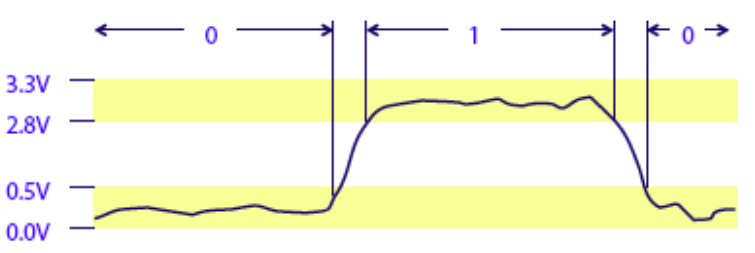
\includegraphics[scale=.5]{images/electric_binary}
\end{center}
\end{figure}

En 1939, Claude Shannon a été le premier à faire un parallèle entre l'algèbre booléenne (une algèbre binaire, n'acceptant que vrai et faux comme valeurs, et trois fonctions logiques “Et (*), Ou(+), Non(-)”) et le fonctionnement des circuits électriques. Le vrai/faux se transforme en 1 : le courant passe, 0 : il ne passe pas. C'est Shannon qui popularise le terme de bit:

\begin{defi}
Le terme {\bf bit} (b minuscule dans les notations) signifie {\it binary digit }, c'est-à-dire 0 ou 1 en numérotation binaire. Il s'agit de la plus petite unité d'information manipulable par une machine numérique. 


L'{\bf octet} (en anglais {\bf byte} ou B majuscule dans les notations) est une unité d'information composée de 8 bits. Il permet par exemple de stocker un caractère comme une lettre ou un chiffre.
\end{defi}

D'autres termes sont aussi utilisés pour définir certaines longueurs de nombre:
\begin{itemize}
\item Une unité d'information composée de 16 bits est généralement appelée {\bf mot} (en anglais {\bf word}).

\item Une unité d'information de 32 bits de longueur est appelée {\bf mot double} (en anglais {\bf double word}, d'où l'appellation dword).
\end{itemize}


\section{Les bases décimales, binaires et hexadécimales}


\subsection{La base décimale}

Le système décimal (base 10) est celui que nous utilisons dans la vie quotidienne parce que nous avons commencé à compter avec nos doigts. Il comporte 10 symboles de 0 à 9. C'est un système positionnel, c'est-à-dire que l'endroit où se trouve le symbole définit sa valeur.

Par exemple: $(9'875)_{(10)}=9 \cdot 10^3 + 8 \cdot 10^2 + 7\cdot 10^1 + 5 \cdot 10^0$

10 représente la base et les puissances de 0 à 3 le rang de chaque chiffre. Quelle que soit la base, le chiffre de droite est celui des unités. Celui de gauche est celui qui a le poids le plus élevé.

\subsection{Binaire}

Dans les domaines de l'automatisme, de l'électronique et de l'informatique, nous utilisons la base 2. Tous les nombres s'écrivent avec deux chiffres uniquement, 0 et 1.  Car l'algèbre booléenne est à la base de l'électronique numérique. Par exemple, un interrupteur est ouvert ou fermé, une diode électroluminescente (ou LED en anglais) est allumée ou éteinte,  une tension est présente ou absente, un champ magnétique est orienté Nord-Sud ou Sud-Nord.

Le chiffre binaire, qui peut prendre ces deux états, est nommé {\bf bit} (binary digit). Les règles sont les mêmes que pour le décimal. 

Par exemple, $1101_{(2)}=1 \cdot 2^3 + 1 \cdot 2^2 + 0 \cdot 2^1 + 1\cdot 2^0=13_{(10)}$ 

\subsubsection{Conversion binaire décimale}

Une méthode pour obtenir le nombre en base 10, connaissant son écriture en base 2, est d'établir la valeur de chaque chiffre du nombre: celui le plus à droite représente 1, le deuxième représente 2, le troisième représente $2^2=4$, le quatrième représente $2^3=8$, etc. comme dans la grille ci-dessous :  

\begin{center}
\begin{tikzpicture}
	\draw (-1,1) rectangle (0,0) rectangle (1,1) rectangle (2,0) rectangle (3,1) rectangle (4,0) rectangle (5,1) rectangle (6,0);
	\draw (5.5,0.5) node {$1$};
	\draw (4.5,0.5) node {$2$};
	\draw (3.5,0.5) node {$4$};
	\draw (2.5,0.5) node {$8$};
	\draw (1.5,0.5) node {$16$};
	\draw (0.5,0.5) node {$32$};
	\draw (-.5,0.5) node {$64$};
	
\end{tikzpicture}
\end{center} 

Par exemple si nous voulons connaitre la valeur décimale du nombre 10110, nous établissons d'abord une grille avec les différentes puissances de 2; ensuite, nous plaçons le nombre en binaire sous cette grille en mettant bien le chiffre des unités sous le carré le plus à droite:

\begin{center}
\begin{tikzpicture}
	\draw (-1,1) rectangle (0,0) rectangle (1,1) rectangle (2,0) rectangle (3,1) rectangle (4,0) rectangle (5,1) rectangle (6,0);
	\draw (5.5,0.5) node {$1$};
	\draw (4.5,0.5) node {$2$};
	\draw (3.5,0.5) node {$4$};
	\draw (2.5,0.5) node {$8$};
	\draw (1.5,0.5) node {$16$};
	\draw (0.5,0.5) node {$32$};
	\draw (-.5,0.5) node {$64$};
	
	\draw (5.5,-0.5) node {$0$};
	\draw (4.5,-0.5) node {$1$};
	\draw (3.5,-0.5) node {$1$};
	\draw (2.5,-0.5) node {$0$};
	\draw (1.5,-0.5) node {$1$};
	\draw (0.5,-0.5) node {$ $};
	\draw (-.5,-0.5) node {$ $};
	
%	\draw (-1,0) -- (0,1)
%				(0,0) -- (1,1)
%				(2,0) -- (3,1)
%				(5,0) -- (6,1);
	\draw (-1,-1) rectangle (0,0) rectangle (1,-1) rectangle (2,0) rectangle (3,-1) rectangle (4,0) rectangle (5,-1) rectangle (6,0);
	
\end{tikzpicture}
\end{center}

Il ne reste plus qu'à additionner les nombres des colonnes qui contiennent un 1: $16 + 4 + 2=22$

N.B. : Ce tableau est extensible à l'infini vers la gauche avec les puissances de 2 suivantes.

\begin{exercice}
\'Ecrire en base 10 les nombres suivants:
\begin{multicols}{2}
\begin{enumerate}
\item $101_{(2)}$
\item $10 000_{(2)}$
\item $1111_{(2)}$
\item $10101_{(2)}$
\item $10_{(2)}$
\item $111 000_{(2)}$

\end{enumerate}
\end{multicols}

Vous pouvez utiliser le tableau ci-dessous : 

\begin{center}
\begin{tikzpicture}
	\draw (-3,1) rectangle (-2,0) rectangle (-1,1) rectangle (0,0) rectangle (1,1) rectangle (2,0) rectangle (3,1) rectangle (4,0) rectangle (5,1) rectangle (6,0);
	\draw (5.5,0.5) node {$1$};
	\draw (4.5,0.5) node {$2$};
	\draw (3.5,0.5) node {$4$};
	\draw (2.5,0.5) node {$8$};
	\draw (1.5,0.5) node {$16$};
	\draw (0.5,0.5) node {$32$};
	\draw (-.5,0.5) node {$64$};
	\draw (-3,-4) rectangle (-2,0) rectangle (-1,-4) rectangle (0,0) rectangle (1,-4) rectangle (2,0) rectangle (3,-4) rectangle (4,0) rectangle (5,-4) rectangle (6,0);
	
\end{tikzpicture}
\end{center} 

\end{exercice}

\subsubsection{Conversion décimale binaire}

Pour trouver l'écriture binaire d'un nombre écrit en base 10, il existe principalement deux méthodes. 


\; 

La première méthode consiste à décomposer le nombre en somme de puissance de 2 et à utiliser la grille précédente. 

Plus concrètement, si nous voulons écrite 99 en binaire. La plus grande puissance de 2 que nous pouvons prendre dans 99 est 64 (128, la suivante, est trop grande). Il reste ensuite: 

99-\textbf{64}= 35. Dans 35 on peut mettre 32, et il restera 

35-\textbf{33}= 3. Dans 3 on ne peut ni mettre 16, ni mettre 8, ni mettre 4. On peut mettre 2 :

3-\textbf{2} = 1 Il reste 1. Dans 1 on peut mettre 1 :

1-\textbf{1} = 0

Cela signifie que 99=64+32+2+1. Sur notre grille cela donne:

\begin{center}
\begin{tikzpicture}
	\draw (-1,1) rectangle (0,0) rectangle (1,1) rectangle (2,0) rectangle (3,1) rectangle (4,0) rectangle (5,1) rectangle (6,0);
	\draw (5.5,0.5) node {$1$};
	\draw (4.5,0.5) node {$2$};
	\draw (3.5,0.5) node {$4$};
	\draw (2.5,0.5) node {$8$};
	\draw (1.5,0.5) node {$16$};
	\draw (0.5,0.5) node {$32$};
	\draw (-.5,0.5) node {$64$};
	
	\draw (5.5,-0.5) node {$1$};
	\draw (4.5,-0.5) node {$1$};
	\draw (3.5,-0.5) node {$0$};
	\draw (2.5,-0.5) node {$0$};
	\draw (1.5,-0.5) node {$0$};
	\draw (0.5,-0.5) node {$1$};
	\draw (-.5,-0.5) node {$1$};
	
%	\draw (1,0) -- +(1,1)
%				(2,0) -- +(1,1)
%				(3,0) -- +(1,1)
%				;
	
\end{tikzpicture}
\end{center}

Donc $99_{(10)}=1100011_{(2)}$.


\;

La deuxième méthode consiste  effectuer des divisions successives par 2. Le nombre en binaire se lira à l'aide des restes des différentes divisions:

\begin{figure}[h]
\begin{center}
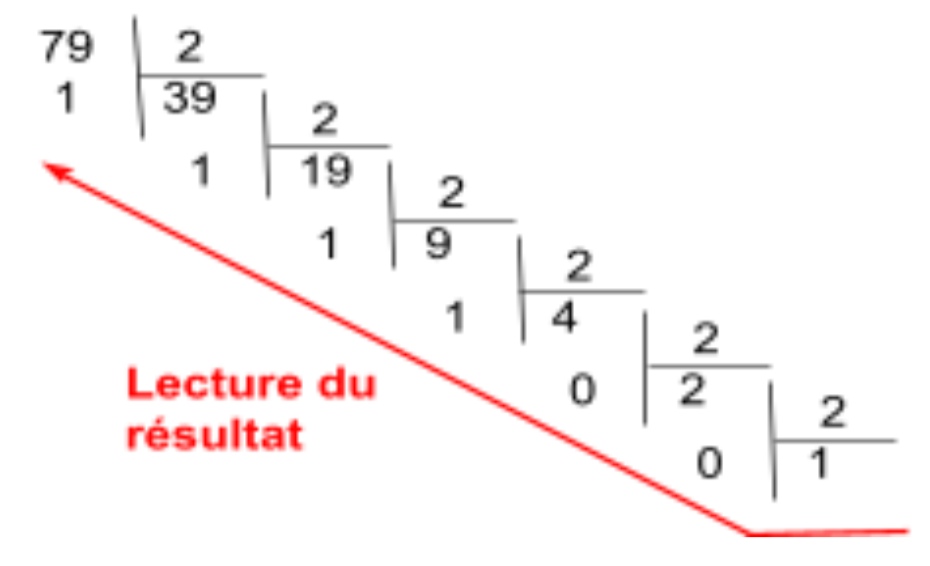
\includegraphics[scale=.5]{images/divisionbinaire}
\end{center}
\end{figure}

Ainsi, $79_{(10)}=1001111_{(2)}$

\begin{exercice}
Les nombres suivants sont écrits en base 10. Donner leur écriture en base 2:
\begin{multicols}{2}
\begin{enumerate}
\item 75
\item 12
\item 27
\item 153
\item 100
\item 200
\item 1000
\item 2000
\end{enumerate}
\end{multicols}
\end{exercice}

\subsection{*La base hexadécimale}

C'est le code utilisé dans la programmation de certains automates et microprocesseurs. Il est composé de : 10 chiffres de 0 à 9, et 6 lettres de A à F. Les adresses MAC (adresses uniques associées à chaque carte réseau dans le monde) sont aussi écrites en base hexadécimale.

La manipulation des nombres écrits en binaire est difficile pour l'être humain et la conversion en décimal n'est pas simple. C'est pourquoi nous utilisons de préférence le système hexadécimal (base 16). 

Le tableau ci-dessous montre la représentation des nombres de 0 à 15 dans les bases 10, 2 et 16.

\begin{figure}[h]
\begin{center}
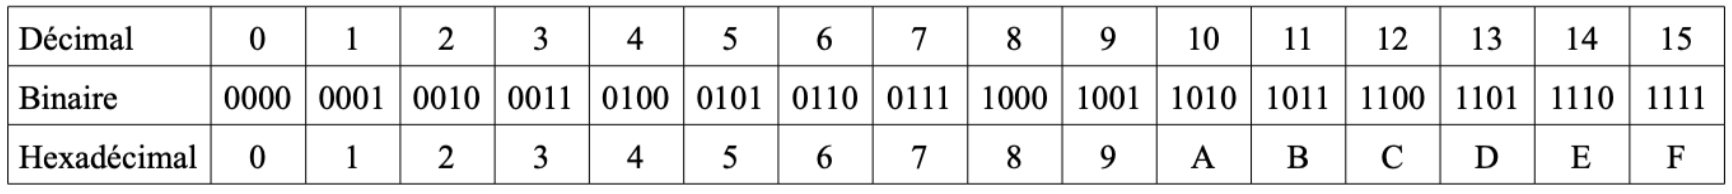
\includegraphics[scale=.5]{images/tableaubase}
\end{center}
\end{figure}


Par exemple, $B4F_{(16)}= B \cdot 16^2 + 4 \cdot 16^1 + F\cdot 16^1= 11 \cdot 16^2 + 4 \cdot 16^1 + 15\cdot 16^0=2 895_{(16)}$

\subsubsection{Conversion en binaire}

Pour convertir un nombre binaire en hexadécimal il suffit de remarquer que chaque groupe de 4 bits représente un chiffre en hexadécimal:

\begin{figure}[h]
\begin{center}
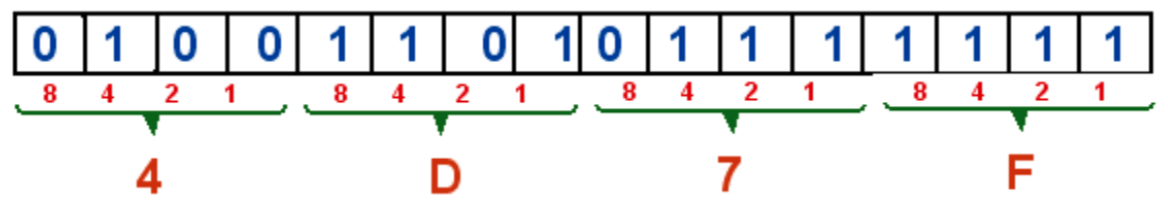
\includegraphics[scale=.5]{images/hexadecimal}
\end{center}
\end{figure}

\begin{exercice}
* Écrire les nombres suivants en base hexadécimale:
\begin{multicols}{2}
\begin{enumerate}
\item $10010010110_{(2)}$
\item $111110_{(2)}$
\item  $1000110101110101_{(2)}$
\item $11110000000011_{(2)}$
\end{enumerate}
\end{multicols}
\end{exercice}

\subsubsection{Conversion en décimal}

La méthode par division (par 16) s'applique comme en binaire (par 2).

\begin{exercice}
* Écrire les nombres suivants en hexadécimal:
\begin{multicols}{2}
\begin{enumerate}
\item 92
\item 256
\item  500
\item 1023
\end{enumerate}
\end{multicols}
\end{exercice}



\subsection{Opération sur les nombres en binaires}

Tout comme pour l'addition en colonne, pour additionner deux nombres écrits en binaires il faut les additionner bit à bit. 

\begin{exercice}
Quel est le résultat des calculs binaires suivants:
\begin{enumerate}[a)]
\item $0+0=$
\ 

\item $1+0=$
\ 

\item $0+1=$
\ 

\item $1+1=$
\ 

\item $1+1+1=$
\end{enumerate}
\end{exercice}

À l'aide de l'exercice suivant effectué l'addition suivante:

$$1100101001 + 101110101$$

Pour cela, compléter l'addition en colonne suivante:

\;

\begin{center}
\begin{tikzpicture}
	\draw (0,0) node{$1$}
				(0.5,0) node{$1$}
				(1,0) node{$0$}
				(1.5,0) node{$0$}
				(2,0) node{$1$}
				(2.5,0) node{$1$}
				(3,0) node{$1$}
				(3.5,0) node{$0$}
				(4,0) node{$0$}
				(4.5,0) node{$1$};
		\draw (-0.5,-.5) node{$+$}
				(0.5,-.5) node{$1$}
				(1,-.5) node{$0$}
				(1.5,-.5) node{$1$}
				(2,-.5) node{$1$}
				(2.5,-.5) node{$1$}
				(3,-.5) node{$0$}
				(3.5,-.5) node{$1$}
				(4,-.5) node{$0$}
				(4.5,-.5) node{$1$};
	\draw (-1,-.8) -- +(6,0);
\end{tikzpicture}
\end{center}

\vskip+1cm

\begin{exercice}
Effectuer les additions binaires suivantes:
\begin{multicols}{2}
\begin{enumerate}
\item $1001 + 101$
\item $10011 + 110011$
\item  $110001 + 11010$
\item $110101 + 101110$
\end{enumerate}
\end{multicols}
\end{exercice}


\begin{exercice}
\begin{enumerate}
\item On voudrait encoder des emojis en binaire; en d'autres mots, on voudrait faire correspondre chaque emoji à un code binaire différent.
\begin{enumerate}
\item Combien peut-on encoder de symboles (ici des emojis) différents sur 3 bits ?
\item Sur 5 bits ?
\item Sur 11 bits ?
\end{enumerate}

\item Combien de nombres peut-on représenter avec 5 bits et avec 12 bits ?

\item Quel est le plus grand nombre qu'on peut écrire sur 8 bits ?


\vspace{10pt}
\item On se pose maintenant la question inverse : 
\begin{enumerate}
\item Combien me faut-il de bits pour encoder 8 symboles différents ?
\item 9 symboles ?
\item 69 symboles ?
\end{enumerate}

\end{enumerate}
\end{exercice}


\section{Représentation des nombres entiers relatifs signés}

{\it Rappel: Les nombres entiers naturels sont l'ensemble des nombres entiers et positifs. Il est désigné par la lettre $\mathbf{N}=\{0,1,2,\ldots\}$.

Les nombres entiers  sont l'ensemble des nombres entiers négatifs et positifs. Il est désigné par la lettre $\mathbf{Z}=\{\ldots,-2,-1.0,1,2,\ldots\}$.}

\ 

Nous arrivons maintenant à écrire tous les nombres entiers naturels en binaire. 

\begin{remarque}

Dans la pratique, nous avons besoin de savoir quelle taille fait chaque nombre, i.e. sur combien de bits, il est codé. On peut par exemple décider que les nombres sont codés sur un octet (8 bits): le plus petit nombre sera 00000000 = 0 et le plus grand sera 11111111=255.
\end{remarque}

{\bf Problème:} En faisant ainsi, nous ne pouvons pas représenter des nombres négatifs.

\ 

Il faut donc utiliser un certain nombre de règles en fonction du type de nombres que l'on veut représenter avec un ordinateur: nombres entiers, nombres relatifs, nombres rationnels...





\subsection{Représentation signe-magnitude}

Une première façon pour représenter les nombres négatifs est de décider que le bit le plus gauche représente le signe du nombre.

\begin{figure}[h]
\begin{center}
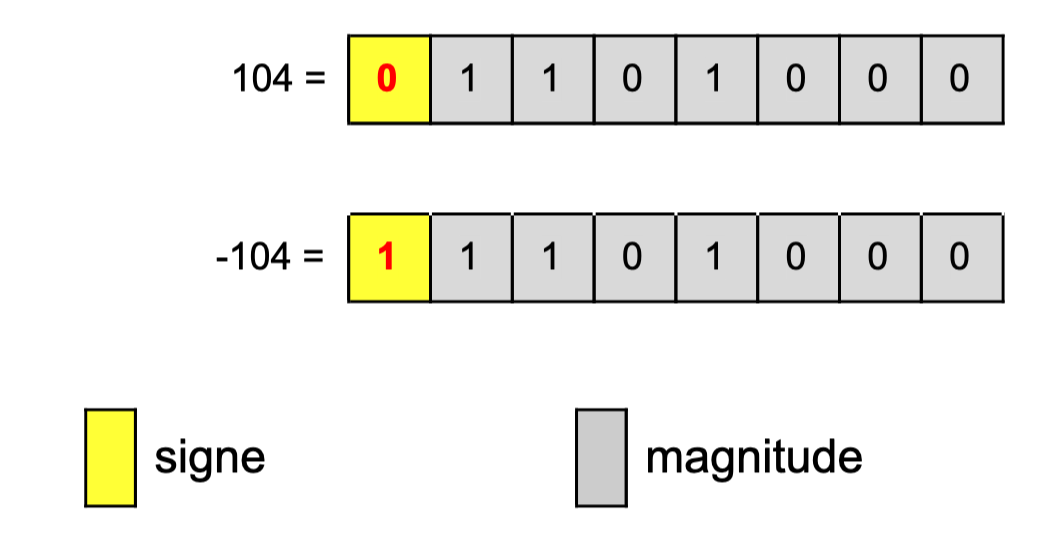
\includegraphics[scale=.5]{images/nombresigne}
\end{center}
\end{figure}

Sur 8 bits, le plus grand nombre représentable sera 01111111=127 et le plus petit sera 111111111=-127.

\ 

Il est possible d'additionner deux nombres pour autant qu'ils soient tous les deux positifs et que le résultat ne dépasse pas le nombre plus grand nombre pouvant être écrit:

\begin{figure}[h]
\begin{center}
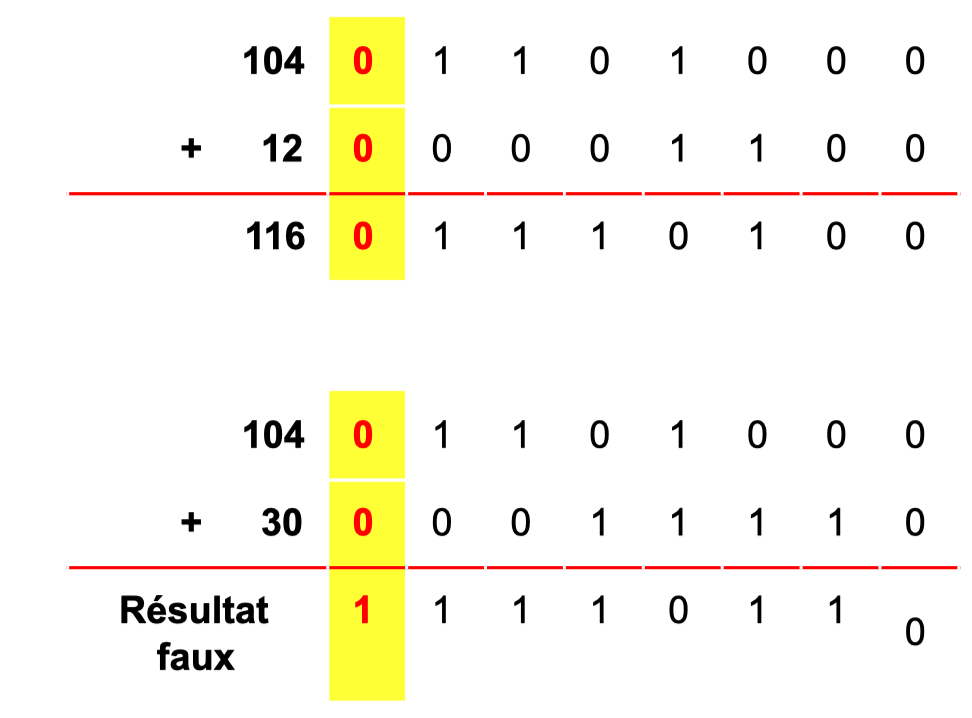
\includegraphics[scale=.5]{images/Operationsigne}
\end{center}
\end{figure}

Le résultat de 104 + 30=134 amène un dépassement de capacité. Le nombre entier signé maximum sur 8 bits est 127.


\ 

{\bf Problème:} Bien que pratique, cette façon de coder les nombres négatifs présente deux problèmes:
\begin{enumerate}
\item zéro est représenté de deux façons différentes: 1000000 et 00000000.
\item si on additionne deux nombres opposés, nous n'obtenons pas 0. 
\end{enumerate}

\subsection{* Représentation des nombres en complément à deux}

Cette représentation résout les problèmes de la représentation signée. Dans cette représentation, pour obtenir l'opposé d'un nombre positif écrit en binaire, nous allons effectuer les deux étapes suivantes:
\begin{enumerate}
 \item On inverse tous les bits du nombre positif (on change les 0 en 1 et inversement). Cela s'appelle le {\bf complément à 1}.
 \item On ajoute 1.
\end{enumerate}

Par exemple, nous aimerions écrire le nombre -80. 

Premièrement, 80 s'écrit en binaire: {\bf 01010000}.

\ 

On prend le complément à 1 de ce nombre, ce qui donne: {\bf 10101111}

\ 

Puis on ajoute 1:

\begin{center}
\begin{tikzpicture}
	\draw (0,0) node{$1$}
				(0.5,0) node{$0$}
				(1,0) node{$1$}
				(1.5,0) node{$0$}
				(2,0) node{$1$}
				(2.5,0) node{$1$}
				(3,0) node{$1$}
				(3.5,0) node{$1$};
		\draw (-0.5,-.5) node{$+$}
				
				(3.5,-.5) node{$1$};
				
		
				
	\draw (-1,-.8) -- +(6,0);
	
	\draw  (0,-1.3) node{$1$}
				(0.5,-1.3) node{$0$}
				(1,-1.3) node{$1$}
				(1.5,-1.3) node{$1$}
				(2,-1.3) node{$0$}
				(2.5,-1.3) node{$0$}
				(3,-1.3) node{$0$}
				(3.5,-1.3) node{$0$};
\end{tikzpicture}
\end{center}

L'avantage de cette méthode est que la somme deux nombres opposés donnera bien 0.

\begin{exercice}
En supposant que les nombres soient écrits sur 8 bits, vérifier que 80 + (-80) = 0.
\end{exercice}

\newpage
\subsection{Résumé}

\begin{figure}[h!]
\begin{center}
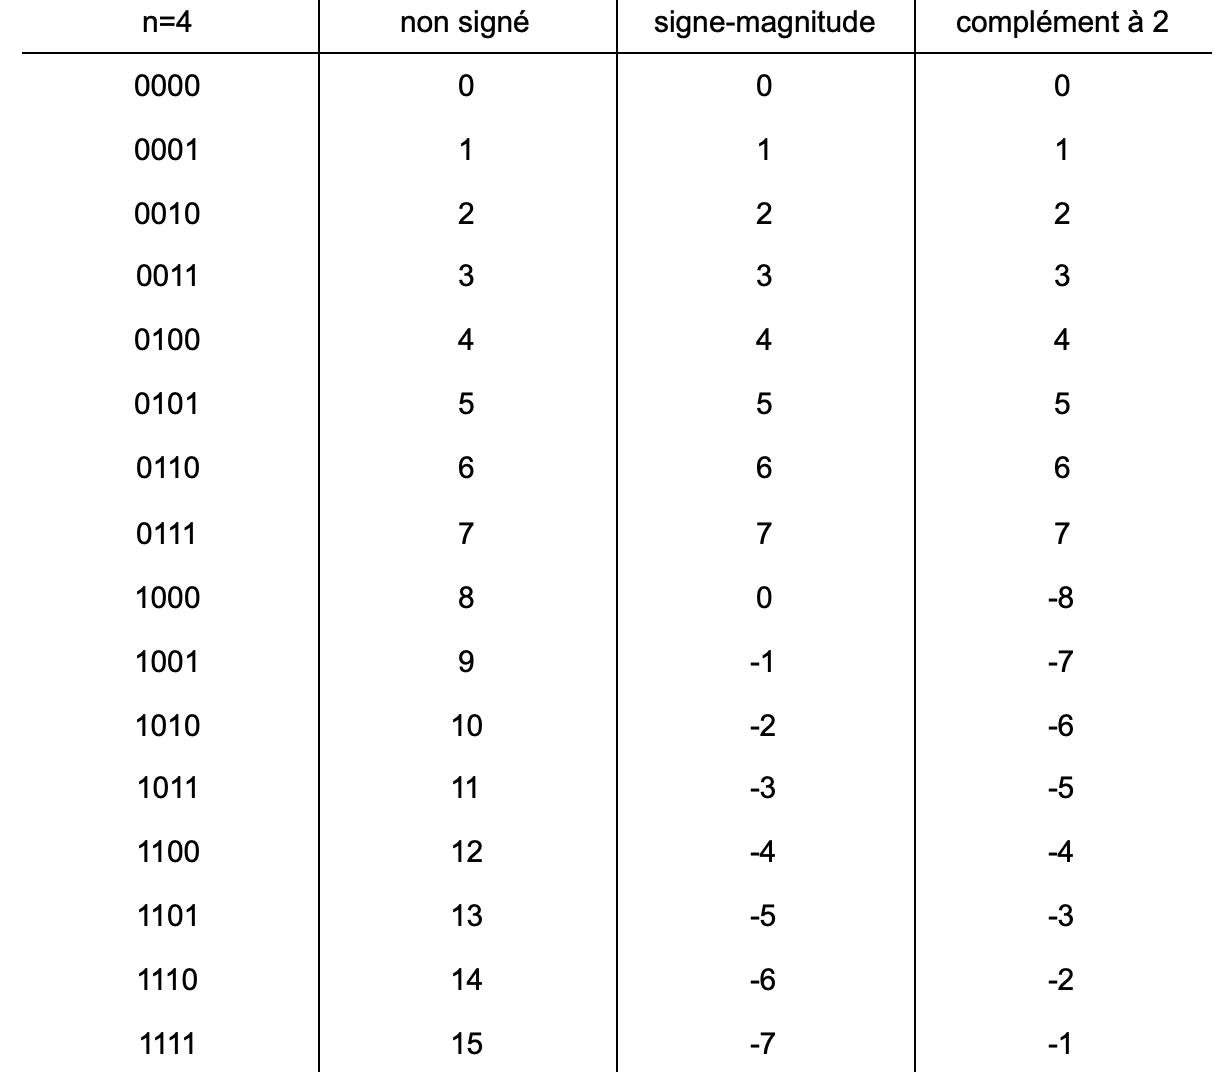
\includegraphics[scale=.45]{images/tablerepresentation}
\end{center}
\end{figure}


%\begin{exercice}
%Utiliser un tableur pour faire une conversion d'une base à l'autre.
%\end{exercice}


\begin{exercice}
Donner la représentation signe-magnitude sur un octet des nombres suivants:
\begin{multicols}{2}
\begin{enumerate}
 	\item -100
 	\item 38
 	\item -200
 	\item -83
\end{enumerate}
\end{multicols}
\end{exercice}


\begin{exercice}\textbf{* Complément à deux }
\begin{enumerate}[a)]
\item Donner la représentation en complément à deux des nombres suivants:

\begin{enumerate}
\item -95
\item -64
\end{enumerate}

\item Vérifier que 95+(-95) donne bien 0 sur un octet.
\item Vérifier que 64+(-6) donne bien 0111010 sur un octet.
\end{enumerate}
\end{exercice}


\begin{exercice}
Nous donnons trois nombres binaires:
\begin{enumerate}[a)]
\item 00101010
\item 1011
\item 10111111
\end{enumerate}

\begin{enumerate}
\item Que valent ces nombres en représentation non signée?
\item Que valent ces nombres en représentation signée?
\item * Que valent ces nombres en complément à 2?
\end{enumerate}
\end{exercice}



\newpage
\section{Les codes de caractères}

\subsection{La table ASCII}

\begin{center}
\begin{figure}[h!]
\centerline{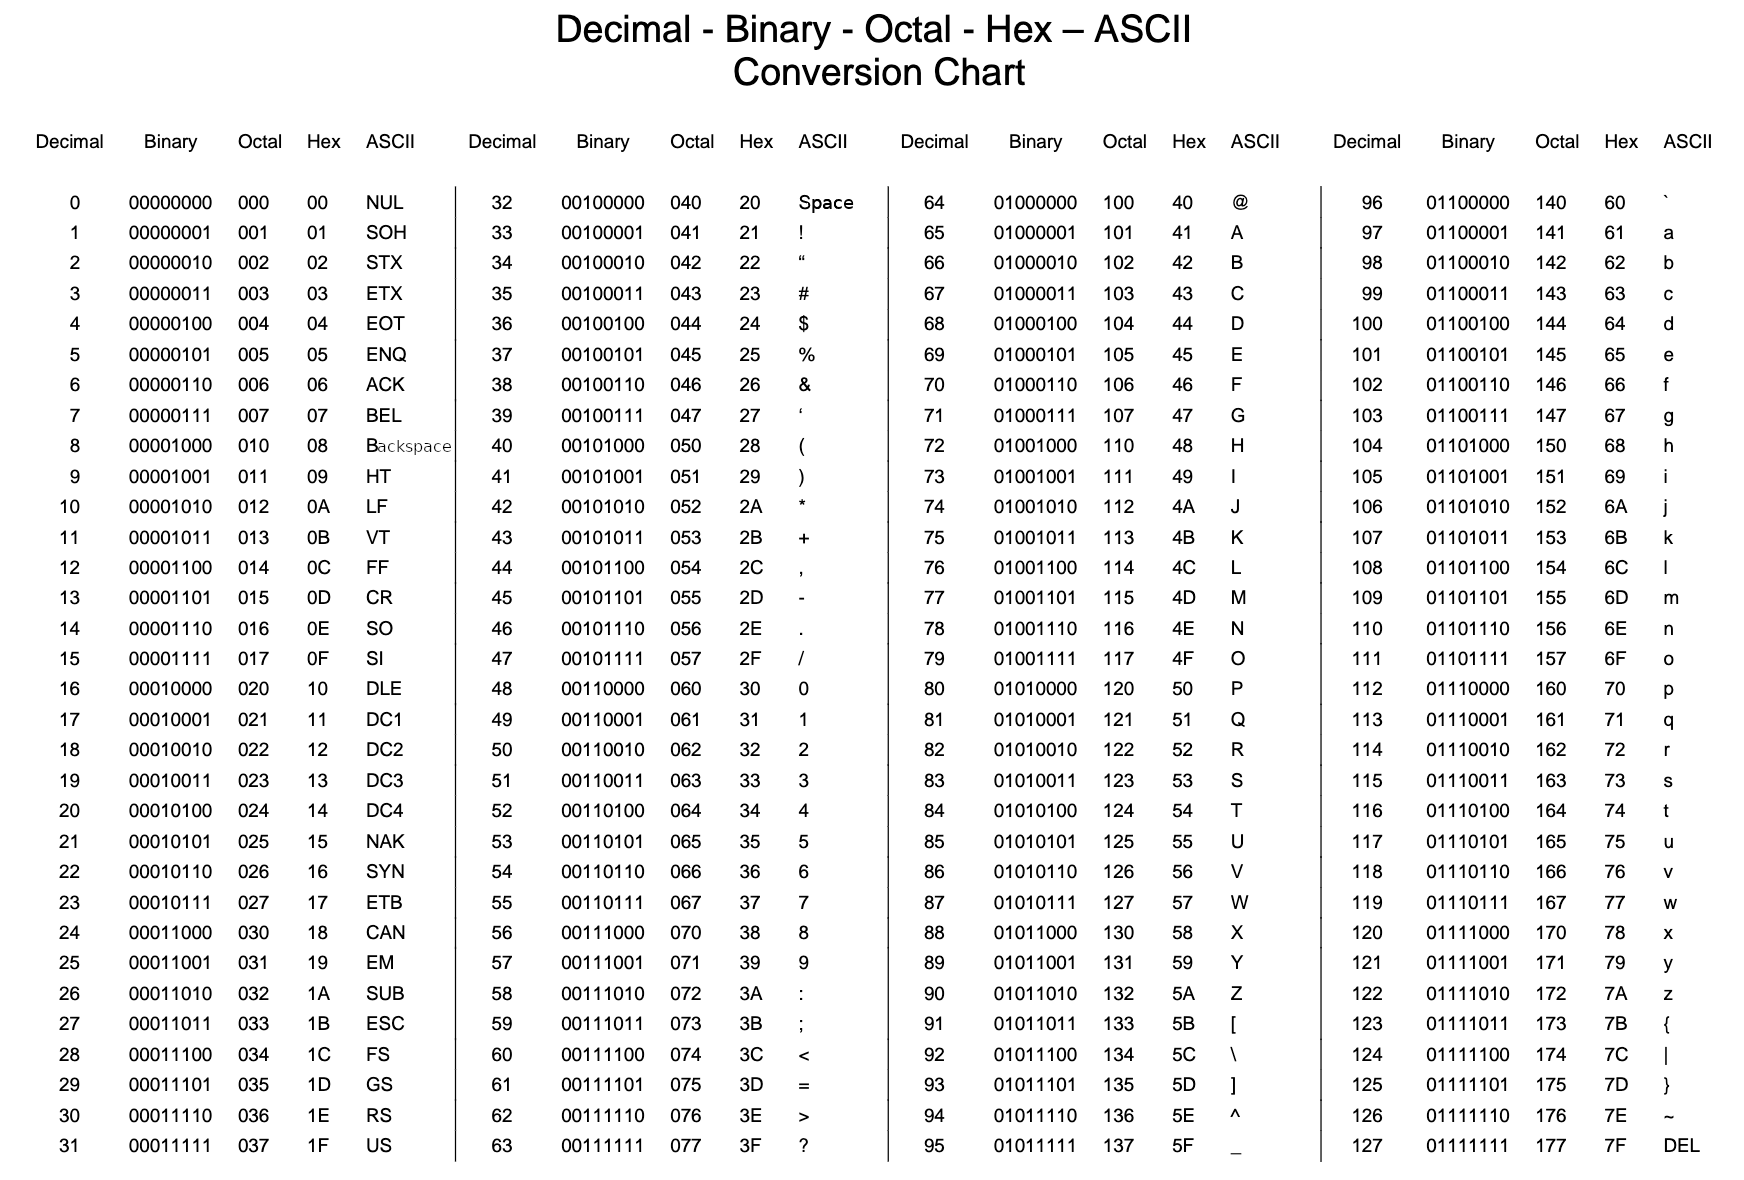
\includegraphics[width=18cm]{images/ASCII2}}
\end{figure}
\end{center}

Le binaire permet de coder les nombres que les systèmes informatiques peuvent manipuler. Cependant, l'ordinateur doit aussi utiliser des caractères alphanumériques pour mémoriser et transmettre des textes par exemple de l’ordinateur vers l’imprimante, d’un automate programmable vers un terminal, d’un clavier vers un processeur, etc. 

Le code {\bf ASCII} (American Standard Code for Information Interchange) représente les caractères sur 7 bits (c'est-à-dire 128 caractères possibles, de 0 à 127). Les codes 0 à 31 ne sont pas des caractères. On les appelle caractères de contrôle car ils permettent de faire des actions telles que : retour à la ligne (CR). Bip sonore (BEL). Les codes 65 à 90 représentent les majuscules. Les codes 97 à 122 représentent les minuscules. Le caractère A par exemple à pour code 65 soit 01000001 en binaire. 


Par exemple: 
\begin{enumerate}[a)]
\item Le caractère f : 102 
\item le point d'interrogation ? : 63 
\item Le chiffre 2 : 50
\end{enumerate}

Le code ASCII a été mis au point pour la langue anglaise, il ne contient donc pas de caractères accentués, ni de caractères spécifiques à une langue. Le code ASCII a donc été étendu à 8 bits pour pouvoir coder plus de caractères (on parle d'ailleurs de code \textbf{ASCII étendu}...)

\subsection{Unicode}

Le code ASCII est utilisable pour l'anglais mais limité pour les autres langues. Il n'y a que 95 caractères imprimables.

Le code Unicode est un système de codage des caractères sur 16 bits mis au point en 1991. Le système Unicode permet de représenter n'importe quel caractère par un code sur 16 bits, indépendamment de tout système d'exploitation ou langage de programmation (environ 64 000 caractères).

Il regroupe ainsi la quasi-totalité des alphabets existants (arabe, arménien, cyrillique, grec, hébreu, latin, ...) et est compatible avec le code ASCII.

L'ensemble des codes Unicode est disponible sur le site {\bf http://www.unicode.org}.


\subsection{Exercices}
\begin{exercice}
Coder ASCII étendu binaire les textes :
\begin{multicols}{2}
\begin{enumerate}
\item { Sismondi}
\item { Cc cv ?}
\end{enumerate}
\end{multicols}
\end{exercice}

\begin{exercice}
Décoder en lettres les mots suivants qui sont codés en ASCII étendu (binaire):
\begin{enumerate}
\item 01100011 01101111 01110101 01100011 01101111 01110101
\item 01001000 01100101 01101100 01101100 01101111 00100000 01110111 01101111 01110010 01101100 01100100 00100000 00100001
\end{enumerate}
\end{exercice}

\begin{exercice}
    En utilisant le codage ASCII étendu, combien d'octets seraient nécessaires pour stocker la phrase suivante:  \texttt{Bonjour l’univers !}
\end{exercice}

\begin{exercice}
* En s’aidant de la table ASCII, classer par ordre croissant les caractères suivants (ne pas tenir compte des virgules) : ESC, A, NUL, Delete, m, 8, <, a, ?
\end{exercice}


\begin{exercice}
* Complétez le tableau ci-dessous:

\begin{figure}[h!]
\begin{center}
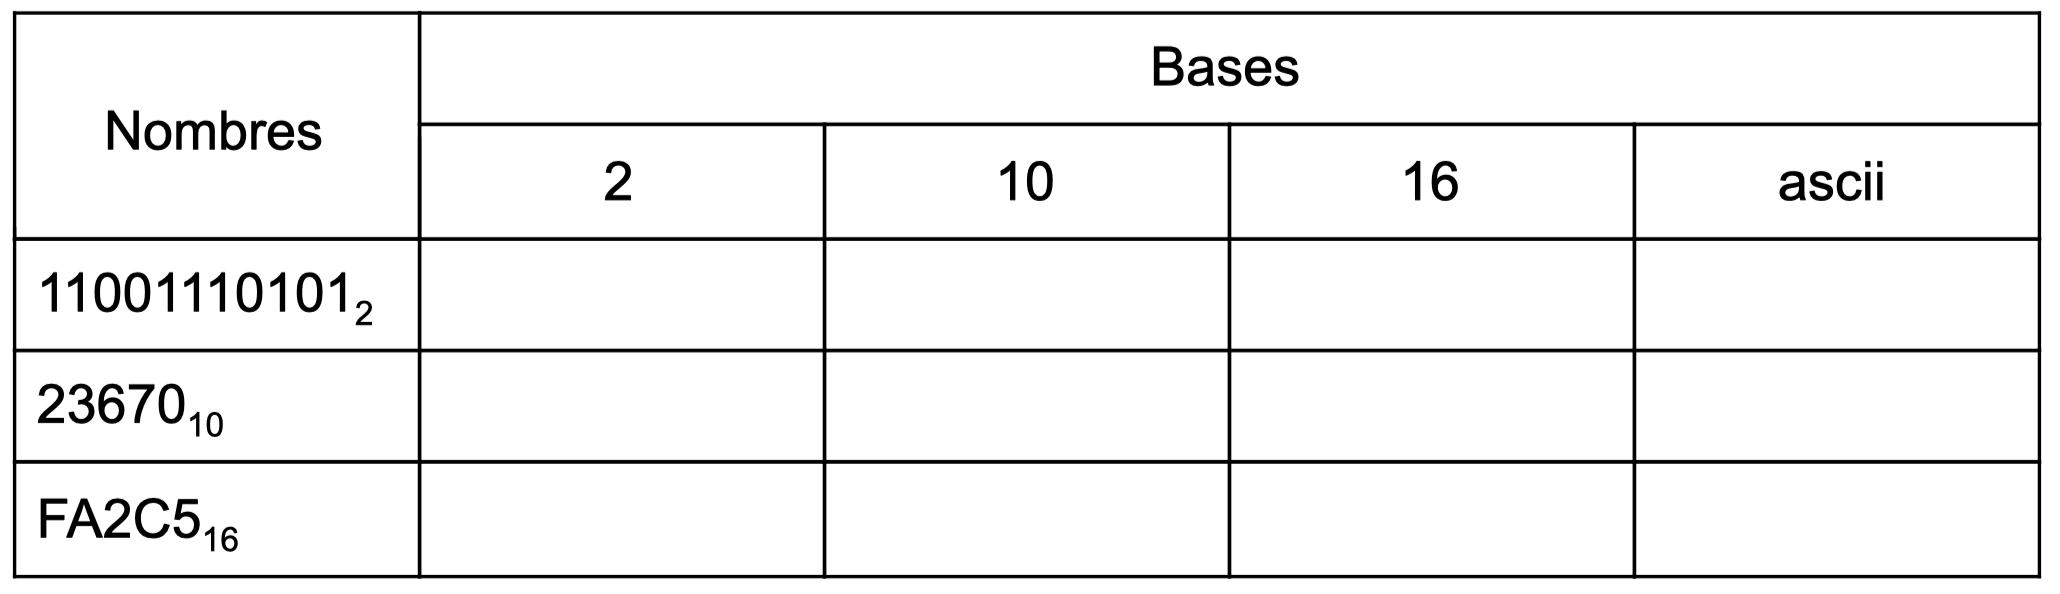
\includegraphics[scale=.25]{images/tableauconversion}
\end{center}
\end{figure}
\end{exercice}

\subsection{Annexe - Table ASCII étendue}
\includepdf[pages=-]{images/3_Table-ASCII_étendue_MS.pdf}
\end{document}
